\documentclass{beamer}
\usepackage{beamerthemesplit}
\usepackage{graphics}
%\usepackage[lined,boxed]{algorithm2e}
\usepackage[lined,noend]{algorithm2e}
\usepackage{amsmath}
\usepackage{amssymb}
\usepackage{listings}
\usepackage{soul}
\usepackage{mathtools}
\usepackage{colortbl}
\usepackage{tikz}
\usepackage{fp}
\usetikzlibrary{calc}

\makeatletter
\newcolumntype{W}{!{\smash{\vrule
\@width 4\arrayrulewidth
\@height\dimexpr\ht\@arstrutbox+2pt\relax
\@depth\dimexpr\dp\@arstrutbox+2pt\relax}}}
\makeatother
\definecolor{gray}{rgb}{.7,.7,.7}



\DeclarePairedDelimiter\ceil{\lceil}{\rceil}
\DeclarePairedDelimiter\floor{\lfloor}{\rfloor}

\lstset{
basicstyle=\small,
keywordstyle=\color{blue}\bfseries,
numbers=left,
numberstyle=\tiny,
numbersep=5pt,
showstringspaces=false,
showspaces=false,
captionpos=b,
frame=tb,
float=tbh,
,escapeinside={*@}{@*}
}
\usetheme{Boadilla}
\title{ Analysis of Algorithms}
\subtitle{Class NP}
\author{Hikmat Farhat}
%\email{hfarhat@ndu.edu.lb}
%\institution{Notre Dame University}
\newtheorem{mydef}{Definition}
\newtheorem{lem}{Lemma}
%\newcommand{\emphasis}[1]{\textcolor{yellow}{#1}}
%\newcommand{\emphasis}[1]{\hl{#1}}
\newcommand{\emphasis}[1]{\ul{#1}}
%\newcommand{\floor}[1]{\lfloor{#1}\rfloor}
%\newcommand{\bfloor}[1]{\Big\lfloor{#1}\Big\rfloor}

%\newcommand{\gets}[0]{\leftarrow}

%\newcommand{\gets}{\ensuremath{\leftarrow}}
%\DeclareTextFontCommand{\emph}{\emphasis}
\sethlcolor{yellow}
\begin{document}

% title page
\frame{\titlepage}

\section{Decision Problems}

\begin{frame}
  \frametitle{Hamiltonian Cycle}
  \begin{itemize}
  \item A Hamiltonian cycle in a graph $G=(V,E)$ is a sequence of non-repeating vertices (except the first and last) such that each pair of vertices are connected in the graph.
  \item For example one Hamiltonian cycle in the graph below is the sequence $s,t,y,x,z,s$ (there are others, e.g.  $s,y,t,x,z,s$)
  \end{itemize}
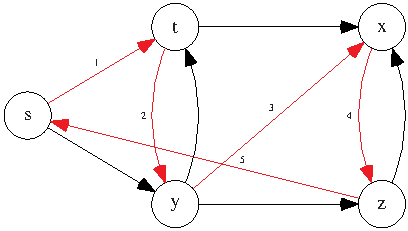
\includegraphics[width=0.7\textwidth]{np-figs/hamiltonian-example}

\end{frame}



\begin{frame}[fragile]
  \frametitle{Decision Problems}

  \begin{itemize}
 \item While the graph in the previous slide contains multiple Hamiltonian cycles, the one below does not contain \textbf{any}
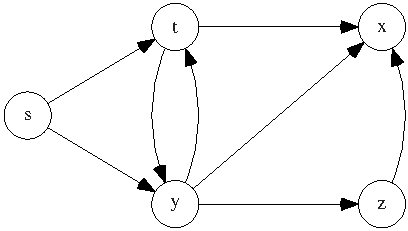
\includegraphics[width=0.7\textwidth]{np-figs/not-hamiltonian}
\item The question of whether a graph contains a Hamiltonian cycle is called a \textbf{decision problem}.

\end{itemize}
\end{frame}

\begin{frame}[fragile]
\frametitle{Formally}
\begin{itemize}
 \item Define the set $H$ as:
  \item $H=\{\text{the set of all graphs } G | G\text{ has a Hamiltonian cycle}\}$
  \item Then given a graph $x$ we need to decide if $x\in H$ or $x\notin H$.
  \item To do so we need an algorithm $A$ that takes a graph $x$ as input and outputs \textbf{yes or no} depending on whether $x\in H$ or not:
    \begin{enumerate}
    \item $A(x)=yes$ then $x\in H$
    \item $A(x)=no$ then $x\notin H$
    \end{enumerate}
\item One can find an algorithm $A$ to solve the problem but, unfortunately, no one has been able to find an \textbf{efficient} one.
\item In fact there are many interesting(decision and optimization) problems that no one has found an efficient algorithm for yet.
  \end{itemize}
% \begin{lstlisting}
% bool binarySearch(int *A,int l,int r,int x){
%    int m=(l+r)/2;

%    if(x==A[m])return true;
%    if(x>A[m]) 
%       return binarySearch(A,m+1,r,x);
%    else 
%       return binarySearch(A,l,m-1,x);
% }
% \end{lstlisting}
%   \begin{itemize}
%   \item The complexity of the above code obeys the recurrence 
%     \begin{align*}
%       T(n)=T(\frac{n}{2})+\Theta(1)
%     \end{align*}
% \item The solution of the recurrence (see Master theorem later) is $T(n)=\Theta(\log n)$.
%   \end{itemize}
\end{frame}

\begin{frame}
  \frametitle{Decision vs Optimization problems}
  \begin{itemize}
  \item Some problems are not decision problems, rather, they can be classified as optimization problems, e.g.  the maximal independent set. 
  \item Given a graph $G=(V,E)$ an independent set is a subset $S\subseteq V$ of vertices such that for all $u,v\in S$ we have $(u,v)\notin E$.
  \item In the graph below $\{t,z\}$ is I.S. as is  $\{y,x\}$ but we want the \textbf{largest} one i.e.  $\{s,x,z\}$
  \end{itemize}
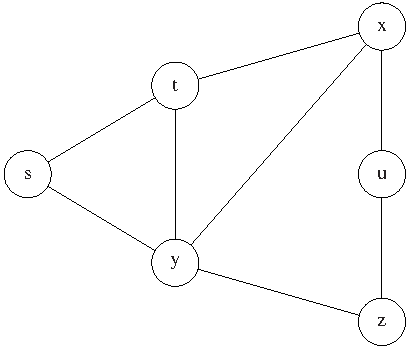
\includegraphics[width=0.5\textwidth]{np-figs/independent}

\end{frame}


\begin{frame}
  \begin{itemize}
  \item Any optimization problem, like the maximal independent set, can be recast as a sequence of decision problems.
  \item In the case of the I.S. in the previous graph we convert it into a sequence of decision problems:
  \item We know there is always an IS of size 1
 \item Is there an IS of size 2? yes
  \item Is there an IS of size 3?yes
 \item IS there an IS of size 4? no
  \item Therefore the maximal independent set has size 3.
\item Note: since the size of the independent set cannot be more that $|V|=n$ then if the decision problem has a polynomial time algorithm then the optimization problem will also have a polynomial time algorithm.
  
  \end{itemize}
\end{frame}

\begin{frame}
  \frametitle{Verifiers}
  \begin{itemize}
  \item As mentioned before, many of the decision problems do not (yet) have an efficient algorithm.
  \item Can we find a common characteristic for some of these problems?
  \item It turns out that for many of them, if we are given a potential solution, we can \textbf{efficiently verify} that it is indeed a solution.
  \end{itemize}
\end{frame}

\begin{frame}
  \begin{itemize}
  \item Let $H$ be the set of graphs that have a Hamiltonian cycle.
  \item Let $x$ be an encoding of a graph and $s$ be a list of vertices of $x$ (certificate).
  \item $B(x,s)$ is called a \textbf{verifier} of $H$  if the following two conditions hold:

    \begin{enumerate}
    \item for all $x\in H$ $\exists s$ such that $B(x,s)$=yes
\item for all $x\notin H$ and $\forall s$, $B(x,s)=$no 
    \end{enumerate}
  \item If $B$ is a polynomial time algorithm and $|s|=O(|x|^c)$ for some $c$ then $B$ is said to be an \textbf{efficient verifier of} $H$


  \end{itemize}
\end{frame}

\begin{frame}
  \frametitle{Class NP}
  \begin{itemize}
  \item We define the class of problems $NP$ (Non-deterministic polynomial time) as all the problems that have \textbf{efficient verifiers}
 \item As an example, the following polynomial algorithm is an efficient verifier for $H$.
 \item Given a graph $G=(V,E)$ and a list of vertices $L$
\item First check that the first and the last element of $L$ are the same, if not return false
\item Then check that no vertex is repeated in $L$ (except the first and last)
\item Finally check that consecutive vertices are connected in $G$
\item The pseudo-code for the above is given in the next slide.
  \end{itemize}
\end{frame}
\begin{frame}
\frametitle{ Hamiltonian Cycle has efficient verifier:$HC\in NP$}
  \begin{function}[H]
 
  \DontPrintSemicolon
  \SetKwFunction{Verify}{Verify}
  \Verify{$G,L$}
  \BlankLine
\tcc{check first and last vertex are equal}
\If{$L[1]\ne L[n]$}{\Return false\;}
\tcc{check that no vertex is repeated (except first and last)}
\For{$i=1$ \KwTo $n-1$}{
  \For{$j=i+1$ \KwTo $n-1$}{ 
   \If{$L[i]=L[j]$}{
     \Return false\;
    }
  }
}
\tcc{check that consecutive vertices are connected}
\For{$i=1$ \KwTo $n-1$}{
  \If{$(L[i],L[i+1])\notin E$}{
    \Return false\;
 }
}
\tcc{passed all checks, $L$ is a Hamiltonian cycle}
\Return true\;  
\end{function}

\end{frame}

\begin{frame}
  \frametitle{IS has efficient verifier: $IS\in NP$  }
  \begin{itemize}
      \item Given a graph $G=(V,E)$ the following polynomial time algorithm verifies that
       $L$ is an independent set of size $k$
  \end{itemize}
  \begin{function}[H]
 
  \DontPrintSemicolon
  \SetKwFunction{Verify}{Verify}
  \Verify{$G,L,size$}
  \BlankLine
\tcc{check that size is $k$}
\If{$size\ne k$}{\Return false\;}
\tcc{check that no vertex is repeated  and no two are connected}
\For{$i=1$ \KwTo $n-1$}{
  \For{$j=i+1$ \KwTo $n$}{ 
   \If{$L[i]=L[j]$}{
     \Return false\;
    }
    \If{$(L[i],L[j])\in E$}{
       \Return false\;
       }
  }
}

\tcc{passed all checks, $L$ is an independent set of size $k$}
\Return true\;  
\end{function}

\end{frame}


\begin{frame}
  \frametitle{Boolean Satisfiability}
  \begin{itemize}
  \item A boolean formula is an expression made of boolean variables that can be assigned the values of TRUE or FALSE  ( 0 or 1), boolean operators $\land$ (conjunction),$\lor$ (negation),$\lnot$ (disjunction) and possibly parenthesis.
\item A \textbf{literal} is a variable or a negation of a variable (i.e. $x$ or $\lnot x$).
\item A \textbf{clause} is a disjunction of literals (or a single literal).
  \item A boolean formula is said to be satisfiable if there is an assignment to the variables such that the expression evaluates to true.
\item The \textbf{boolean satisfiability problem} (\textbf{SAT}) is the problem of deciding whether a boolena formula is satisfiable.


\item A special case of SAT is \textbf{ 3SAT}, when the formula is formed by a conjunction of clauses, where each clause has at most three literals 
  \end{itemize}
\end{frame}
\begin{frame}
  \frametitle{$SAT,3SAT\in NP$}
  
  \begin{itemize}
   \item Let $n$ be the number of variables and  $k$ be the number of clauses. The double array $F[i][j]$ gives the index of variable $j$ in clause $i$.
  \item For example $F[2][3]=7$ means that the third variable in clause 2 is $x_7$
  \item $A[i]$ is the value (0 or 1) assigned to variable $x_i$
   \item The following is an efficient verifier for 3SAT where $A$ is an array of size $n$ containing the value of the $n$ boolean variables (assignment)
  \end{itemize}
 \end{frame}

\begin{frame}
\frametitle{Efficient verifier for $3SAT$}
 \begin{function}[H]
 
  \DontPrintSemicolon
  \SetKwFunction{Verify}{Verify}
  \Verify{$F,A$}
  \BlankLine

\tcc{check that each clause is satisfied}
\For{$i=1$ \KwTo $k$}{
  $sum\gets 0$\;
  \For{$j=1$ \KwTo $3$}{ 
   $sum\gets sum+A[F[i][j]]$\;
   }
   \If{$sum=0$}{
     \Return false\;
    }
}
\tcc{all clauses are satisifed }
\Return true\;  

\end{function}
\end{frame}

\begin{frame}
  \frametitle{Example}
  \begin{itemize}
  \item Consider the following $3SAT$ formula with three clauses and five variables
    \begin{align*}
      \left(x_1\lor x_2\lor\lnot x_5  \right) \land \left(x_3\lor\lnot x_2\lor\lnot x_4  \right)\land \left(\lnot x_4\lor\lnot x_3\lor\lnot x_2  \right)
    \end{align*}
\item The formula is satisfied with the assignment $x_1=1,x_2=0$ (regardless of the values of $x_3$,$x_4$ and $x_5$)
\item One can convince you that the formula is satisfiable by supplying a \textbf{short} proof which in this case the assignment of the variables.
 \item You can check (in polynomial time, refer to the previous slides) that the supplied assignment indeed makes the formula satisfiable.
\item Whereas the converse is not true. Consider the formula below 
  \end{itemize}
\end{frame}

\begin{frame}
 \frametitle{Unsatisfiable formula}
    \begin{itemize}
    \item  How can one convince you that the formula below is unsatisfiable? Can they supply a \textbf{short} proof?
   \item You have to check all possibilities 
    \end{itemize}

    \begin{align*}
      &\left(x_1\lor x_2\lor x_3  \right) \land \left(x_1\lor\lnot x_2\right)\land \left( x_2\lor\lnot x_3 \right)\land\left(x_3\lor \lnot x_1\right)      \land &\left(\lnot x_1\lor\lnot x_2\lor\lnot x_3 \right) 
    \end{align*}

\end{frame}

\section{Using Z3}

\begin{frame}
  \frametitle{Using Z3}
  \begin{itemize}
  \item Even though SAT is NP-complete, which means no polynomial time algorithm exists yet for solving it, many SAT solvers are very efficient solvers of SAT
  instances
\item They use backtracking (later) and heuristics.
  \item We will give examples using \textbf{Z3}
  \item The input to Z3 is a set of disjunctive clauses. This means that the input formula is a conjunctive normal form (CNF).
  \end{itemize}
\end{frame}
\begin{frame}[fragile]
  \frametitle{Example1}
  \begin{itemize}
  \item The satisfiable formula below
 \begin{align*}
      \left(x_1\lor x_2\lor\lnot x_5  \right) \land \left(x_3\lor\lnot x_2\lor\lnot x_4  \right)\land \left(\lnot x_4\lor\lnot x_3\lor\lnot x_2  \right)
    \end{align*}
\item Is input into a file, say formula.cnf, for Z3 as follows
  \end{itemize}

\begin{verbatim}
(declare-const x1 Bool)
(declare-const x2 Bool)
(declare-const x3 Bool)
(declare-const x4 Bool)
(declare-const x5 Bool)
(assert (and 
          (or x1 x2 (not x5))
          (or x3 (not x2) (not x4))
          (or (not x4) (not x3) (not x2))
        )
)
(check-sat)
(get-model)
\end{verbatim}

\end{frame}
\begin{frame}[fragile]
  \begin{itemize}
  \item run "z3 formula.cnf". The first line says "sat" which means the formula is satisfiable and then it prints the assignment.
  \end{itemize}

\begin{verbatim}
  sat
  (model
    (define-fun x3 () Bool
      false)
    (define-fun x2 () Bool
      false)
    (define-fun x1 () Bool
      false)
    (define-fun x5 () Bool
      false)
    (define-fun x4 () Bool
      false)
  )
\end{verbatim}
\end{frame}
\begin{frame}[fragile]
  \begin{itemize}
  \item The unsatisfiable formula
  \end{itemize}
\begin{align*}
      &\left(x_1\lor x_2\lor x_3  \right) \land \left(x_1\lor\lnot x_2\right)\land \left( x_2\lor\lnot x_3 \right)\land\left(x_3\lor \lnot x_1\right)      \land &\left(\lnot x_1\lor\lnot x_2\lor\lnot x_3 \right) 
    \end{align*}
    \begin{itemize}
    \item Is written as 
    \end{itemize}
\begin{verbatim}
(declare-const x1 Bool)
(declare-const x2 Bool)
(declare-const x3 Bool)
(assert (and 
          (or x1 x2 x3)
          (or x1 (not x2) )
          (or x2 (not x3) )
          (or  x3 (not x1))
          (or (not x1) (not x2) (not x3))
        )
)
(check-sat)
(get-model)
\end{verbatim}
\end{frame}
\begin{frame}[fragile]

\begin{itemize}
  \item when we run z3 on the above input we get
\end{itemize}
\begin{verbatim}
  unsat
  (error "line 13 column 10: model is not available")
\end{verbatim}
\end{frame}

\section{Polynomial Time Reduction}
\begin{frame}
  \frametitle{Polynomial time reductions}
  \begin{itemize}
  \item Let $Y$ and $X$ be decision problems.
  \item We say that $Y$ is polynomial time reducible to $X$, and write $Y\le_pX$ if
  \item If there exists a function (or procedure) $f$ such that 
    \begin{enumerate}

   \item $f$ is polynomial time
   \item $v\in Y\Leftrightarrow f(v)\in X$
    \end{enumerate}
\item The importance of reduction is that if one has a polynomial time algorithm for $X$ it can be used to solve instances of $Y$ in polynomial time.
  \end{itemize}
\end{frame}
\begin{frame}
  As shown in the figure below, a reduction $f$ maps all instances in $X$ to instances in $Y$ 
  and all instances not in $X$ to instances not in $Y$.
  \begin{tikzpicture}
    \draw (0,0) ellipse (1 and 1.5);
    \draw (4,0) ellipse (1 and 1.5);
    \draw (3,0)--(5,0);
    \node(Y) at (4,0.5){$Y$};
    \node(nY) at (4,-0.5){$\neg Y$};
    \draw (-1,0)--(1,0);
    \node(X) at (0,0.5){$X$};
    \node(nX) at (0,-0.5){$\neg X$};
    \draw[->] (X)--(Y)[dashed] node [midway,above]{$f$};
    \draw[->]  (nX)--(nY)[dashed] node [midway,above]{$f$};
  \end{tikzpicture}
\end{frame}
\begin{frame}
  \begin{itemize}
  \item Theorem: If $Y\le_p X$ and $X\in P$ then $Y\in P$. 
\item \textbf{Proof.}
\item $X\in P$ then there exists a polynomial time algorithm  $B$ that decides $X$. This means 
that for any $u$, $B(u)=True \Leftrightarrow u\in X$.
\item $Y\le_p X$ then there exists a polynomial time function $f$ such that $v\in Y\Leftrightarrow f(v)\in X$.
\item Let $v$ be any instance. Compute $f(v)=u$ in polynomial time.
\item Decide $u$ in polynomial time using $B$
\item $B(u)=$true then $f(v)=u\in X$ and therefore $v\in Y$ return true
\item $B(u)=$false then $f(v)\notin X$ and therefore $v\notin Y$ return false
\item The above is a procedure to decide in polynomial time any instance $y$ of $Y$ and thus $Y\in P$.
\item We are actually more interested in the \textbf{contrapositive}
  \end{itemize}
\end{frame}

\begin{frame}
\frametitle{Hard problems}
  \begin{itemize}

  \item Theorem: If $Y\le_p X$ and $Y\notin P$ then $X\notin P$.
\item Proof.
\item By contradiction. Assume that $X\in P$ then there exists a polynomial time algorithm to decide $X$. 
\item Since $Y\le_P X$ then using the previous theorem we know there exists a polynomial time algorithm to decide $Y$ which is a contradiction since $Y\notin P$.
\item The above theorem gives us a notion of "hardness" of a problem.
\item $Y\le_P X$ can be interpreted that $X$ is at least as "hard" to solve as $Y$.
\item This observation lead us to the important class of problems called NP-complete.
  \end{itemize}
\end{frame}
\begin{frame}
  \frametitle{NP-complete Problems}
  \begin{itemize}
  \item A problem $X$ is said to be NP-complete if
    \begin{enumerate}
    \item $X\in NP$
   \item For all $Y\in NP$ we have $Y\le_p X$.
    \end{enumerate}
\item So in a sense NP-complete problems are the "hardest" problems in NP.
\item So far we have shown the following relations
  \begin{enumerate}
  \item $P\subseteq NP$
  \item NP-complete $\subseteq NP$.
  \end{enumerate}
\item But are $P$ and NP-complete proper susbsets of $NP$ ?
\item Most researchers believe so, but it hasn't been proved yet!
  \end{itemize}

\end{frame}


\begin{frame}
  \frametitle{SAT is NP-complete}
  \begin{itemize}
   \item Theorem (Cook 1971): SAT is NP-complete.

   \item We will use 3SAT as our starting point to show some of well known problems to be NP-complete 
  \end{itemize}
\end{frame}

\section{SAT to 3SAT}

\begin{frame}
  \frametitle{SAT to 3SAT}
  \begin{itemize}
  \item Any formula $\phi$ in CNF  can be transformed into a formula $\psi$ in CNF with each clause having at most three literals such that $\psi$ is satisfiable iff $\phi$ is satisfiable. 
\item The transformation works as follows:
  \begin{enumerate}
  \item Given a clause $C=(l_1\vee l_2\vee A)$ where $l_1$ and $l_2$ are literals and $A$ is a disjunction of $k$ literals.
  \item Introduce a new variable $y$ and convert $C$ into $C'=(l_1\vee l_2\vee y)\wedge (\bar{y}\vee A)$
  \item Note we started with a clause that has $k+2$ literals into two clauses of size $3$ and $k+1$.
   \end{enumerate}
  \end{itemize}
\end{frame}

\begin{frame}
  \frametitle{Correctness}
  \begin{itemize}
  \item Suppose that $(l_1\vee l_2\vee A)$ is satisfiable then
    \begin{enumerate}
    \item Either $(l_1\vee l_2)$ is satisfiable then set $y=0$ so $(l_1\vee l_2\vee y)\wedge(\bar{y}\vee A)$ is satisfiable.
    \item Or $A$ is satisfiable then set $y=1$ so $(l_1\vee l_2\vee y)\wedge(\bar{y}\vee A)$ is satisfiable.
    \end{enumerate}
  \item Suppose that $(l_1\vee l_2\vee y)\wedge (\bar{y}\vee A)$ is satisfiable then
    \begin{enumerate}
    \item $l_1$, $l_2$ and $A$ cannot all be false, i.e. one of them is true so $(l_1\vee l_2\vee A)$ is satisfiable.
    \end{enumerate}
  \end{itemize}
\end{frame}

\begin{frame}
  \begin{itemize}
  \item Let $A=l_3\vee B$ then we have ($B$ has $k-1$ literals)
    \begin{align*}
      (l_1\vee l_2\vee y)\wedge (\bar{y}\vee l_3\vee B)
    \end{align*}
  \item We repeat our construction one more time by adding a variable $z$
    \begin{align*}
      (l_1\vee l_2\vee y)\wedge (\bar{y}\vee l_3\vee z)\wedge (\bar{z}\vee B)
    \end{align*}
  \end{itemize}
\end{frame}



\begin{frame}
  \begin{itemize}
  \item We repeat the above procedure until no clauses has more than 3 literals.
  \item Since in the original formula each clause has at most $n$ literals we need at most $O(n)$ operations to reduce a clause to at most 3 literals.
  \item Starting from $k$ clauses our procedure is $O(k\cdot n)$, clearly polynomial in the number of variables.
  \item Since SAT is NP-complete and we have a polynomial time reduction from SAT to 3SAT then 3SAT is NP-complete.
  \end{itemize}
\end{frame}

\begin{frame}
  \frametitle{3SAT$\le_p$ Independent Set}
  \begin{itemize}
  \item We prove that a $k$-clause 3SAT decision reduces to $k$-independent set decision.
\item For every literal $x_{ij}$, $i=1,\ldots,k$,$j=1,2,3$, create a graph vertex labeled $x_{ij}$.
\item Nodes representing literals belonging to the same clause are mutually connected (see below for clause $i$)
  \end{itemize}
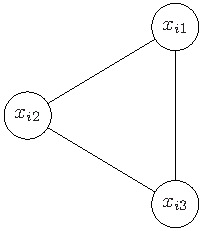
\includegraphics[width=0.3\textwidth]{np-figs/3SAT-to-IS}
\end{frame}
\begin{frame}
  \begin{itemize}
  \item For every literal in clause $i$, $x_{il}$, if its negation occurs in clause $j\ne i$ then the vertices representing these two variables are joined with an edge.
\item Example below where variable $x_{l2}$ in clause $l$ is the negation of $x_{i1}$ in clause $i$
  \end{itemize}
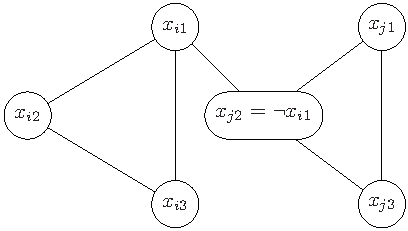
\includegraphics[width=0.5\textwidth]{np-figs/3SAT-to-IS-negation}
\end{frame}

\begin{frame}
  \begin{itemize}
  \item Suppose that a $k$-clause 3SAT instance is satisfiable. Then each clause has at least one variable set to true. Select from each clause
one variable that is set to true to obtain $k$ variables (not necessarily distinct but from different clauses) set to true.
 Now consider the corresponding  set of nodes. Since the 3SAT instance is satisfiable 
the set of variables cannot contain a variable and its complement then  nodes  corresponding to different clauses are not connected. Furthermore, since we chose 
one node (corresponding to a variable) from every clause implies that the chosen set is independent and has size $k$.

\item Suppose that an independent set of $k$ nodes exists. Then the variables corresponding to the nodes do not contain any variable and its negation together therefore it is safe to set the variables to true which implies that each clause of the 3SAT problem has at least one true variable, thus the 3SAT instance is satisfiable
  \end{itemize}
\end{frame}
\begin{frame}
  \frametitle{Example}
  \begin{itemize}
  \item Consider the 3SAT formula 
    \begin{align*}
      \phi=\left(x_1\lor\lnot x_2\lor\lnot x_3\right)\land\left(\lnot x_1\lor x_2\lor x_3\right)\land\left(x_1\lor x_2\lor\lnot x_3\right)
    \end{align*}
\item It is reduced to an instance of IS as shown below
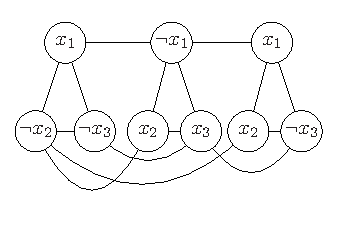
\includegraphics[width=0.9\textwidth]{np-figs/example-3SAT-to-IS}
  \end{itemize}
\end{frame}
\begin{frame}
  \frametitle{Independent Set $\le_p$ Vertex Cover}
  \begin{itemize}
  \item Given a graph $G=(V,E)$ a subset of vertices $S\subseteq V$ is said to be a vertex cover iff for every edge $(u,v)\in E$ either $u\in S$ or $v\in S$.
  \item Usually we look for the \textbf{smallest} vertex cover in a graph.
  \item The corresponding decision problem is: given a graph $G=(V,E)$ is there a vertex cover of size $k$. Clearly $V$ is a vertex cover of size $n$.
  \item We show that deciding vertex cover of size $k$ is NP-complete by reducing it to independent set of size $n-k$.
  
  \end{itemize}

\end{frame}
\begin{frame}
  \frametitle{Proof}
  \begin{itemize}
  \item Suppose that $S$ is a vertex cover. We need to show that $V-S$ is an independent  set.
  \item Assume otherwise, then there exists two vertices $u,v\in V-S$ and  $(u,v)\in E$. This implies that   both ends of the edge $(u,v)$ do not belong to $S$ which means that $S$ is not a vertex cover. A contradiction. Therefore  $V-S$ is an independent set.
\item Conversely assume $V-S$ is an independent set. We need to show that $S$ is a vertex cover.
 \item Assumed otherwise, then there exists an edge $(u,v)\in E$ such that both $u\notin S$ and $v\notin S$ hence $u\in V-S$, $v\in V-S$ and $(u,v)\in E$ therefore $V-S$ is not an independent set. A contradiction.
  \end{itemize}
\end{frame}
\begin{frame}
  \frametitle{Independent Set $\le_p$ Clique}
  \begin{itemize}
  \item Given a graph $G=(V,E)$ a clique is a subset of vertices $S\subset V$ such that for any $u,v\in S$ we have $(u,v)\in E$.
  \item Next we describe a polynomial time reduction from Independent set of size $k$ to a clique of size $k$.
  \item Let $G=(V,E)$ be a graph and construct from $G$ a complement  graph  $G^c=(V,E^c)$ such that  $(u,v)\notin E$ iff $(u,v)\in E^c$.
  \item $G$ has an independent set of size $k$ iff $G^c$ has a clique of size $k$.
  \item \textbf{Proof:} Suppose $S$ is an independent set of $G$ of size $k$ we show that $S$ is a clique of $G^c$ of size $k$. Let $(u,v)\in S$, since $S$ is independent set of $G$ then $(u,v)\notin E$ and therefore $(u,v)\in E^c$
  \end{itemize}
\end{frame}

\begin{frame}
  \frametitle{3SAT $\le_p$ Clique}
  \begin{itemize}
  \item Another way of showing that clique is NP complete is a reduction from 3SAT that is similar to the reduction to independent set.
  \item We will use the reduction from independent set to clique as a guide.
  \item For every literal in every clause we create a vertex. Vertices corresponding to literals in the same clause are not connected (opposite for IS). 
Every node representing a literal in clause $i$ is connected to every node representing literal in clause $j\ne i$ unless these literals are complements to each other (again the opposite for IS).
\item The above construction gives us that $3SAT$ with $k$ clauses is satisfiable iff the corresponding graph has a $k$ clique.
  \end{itemize}
\end{frame}

\begin{frame}
  \frametitle{Useful SAT encoding}
  \begin{itemize}
  \item Because SAT solvers are very efficient it convenient to reduce many problems to SAT. 
  \item In the previous section we concentrated on reduce SAT (or 3SAT) to other problems to show them NP-complete.
  \item When looking for a solution usually we would like to perform the opposite reduction.
  \item To do that it is useful to review some convenient SAT encoding of common situations
  \end{itemize}
\end{frame}
\begin{frame}
  \frametitle{At least one, two, three,...}
  \begin{itemize}
  \item Given $n$ boolean variables $x_1,\ldots, x_n$.
  \item One of the common situations is to require at least $k$ of them to be true.
  \item We start with a small example and then we generalize.
  \item Suppose we have three variables $x_1,x_2,x_3$
  \item If we require that \textit{at least one} is true can be written as a single clause $(x_1\vee x_2\vee x_3)$.
  \item what about at least two?three?
  \item At least two $(x_1\vee x_2)\wedge (x_1\vee x_3)\wedge (x_2\vee x_3)$
  \item At least three is just $x_1\wedge x_2\wedge x_3$.
  \end{itemize}
\end{frame}
\begin{frame}
  \frametitle{Generalization}
  \begin{itemize}
  \item For $n$ variables $x_1,\ldots x_n$ at least $k$ requires all combinations of $n-k+1$ variables.
  \item At least two requires all combinations of $n-2+1$
  \item For $x_1,x_2,x_3,x_4$ this means all combinations of 3 variables
    \begin{align*}
     (x_1\vee x_2\vee x_3)\wedge (x_1\vee x_2\vee x_4)\wedge (x_1\vee x_3\vee x_4)\wedge (x_2\vee x_3\vee x_4) 
    \end{align*}
\item At least three requires all combinations of $4-3+1$ variables
  \begin{align*}
    &(x_1\vee x_2)\wedge (x_1\vee x_3)\wedge (x_1\vee x_4)\\
    \wedge&(x_2\vee x_3)\wedge (x_2\vee x_4)\wedge (x_3\vee x_4)
  \end{align*}
  \end{itemize}
\end{frame}
\begin{frame}[fragile]
  \frametitle{Python itertools}
  \begin{itemize}
  \item itertools is a python package that is useful in listing different combinations of variables
  \item for example to list all combination of 2 and 3 variables from a set of 4 variables we can write
  \end{itemize}
\begin{lstlisting}
import itertools
vars=[1,2,3,4]
for (i,j) in itertools.combinations(vars,2):
   print(i,j)

for (i,j,k) in itertools.combinations(vars,3):
   print(i,j,k)

\end{lstlisting}
\end{frame}

\section{IS->SAT}


\begin{frame}
  \frametitle{Solving Indepent set}
  \begin{itemize}
  \item Given a graph $(V,E)$ with $\lvert V\rvert=n$ we would like to determine if there is an independent set of size $k\le n$.
  \item We can reduce this problem to SAT as follows
    \begin{enumerate}
    \item We assign a variable $x_i$ to each node $i$.
    \item Since we are looking for size $k$ then at least $k$ variables should be true
   \item For each edge $(x_i,x_j)$ add a constraint that both of them cannot be true
    \end{enumerate}
  \end{itemize}
\end{frame}
\begin{frame}
  \frametitle{Example}
  \begin{itemize}
  \item The graph below has 4 nodes so we create 4 boolean variables $x_1,x_2,x_3,x_4$.
  \item We are looking for an independent set of size 2 so we need at least two variables to be true: all combinations of 4-(2-1)=3
  \end{itemize}
  \begin{align*}
    (x_1\vee x_2\vee x_3)\wedge (x_1\vee x_2\vee x_4)\wedge (x_1\vee x_3\vee x_4)\wedge (x_2\vee x_3\vee x_4)
  \end{align*}
  \begin{figure}[h]
    \centering
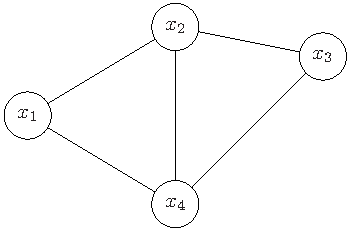
\includegraphics{np-figs/independent2}
  \end{figure}
\end{frame}
\begin{frame}[fragile]
  \begin{itemize}
  \item We also need to add the edge constraints



  \begin{align*}
    (\bar{x}_1\vee \bar{x}_2)\wedge (\bar{x}_1\vee \bar{x}_4)\wedge (\bar{x}_2\vee \bar{x}_3)\wedge (\bar{x}_2\vee \bar{x}_4)\wedge (\bar{x}_3\vee\bar{x}_4)
  \end{align*}
\item The z3 input will look like
  \end{itemize}
  \small{
\begin{verbatim}
  (declare-const x1 Bool)
  (declare-const x2 Bool)
  (declare-const x3 Bool)
  (declare-const x4 Bool)
  (assert (or x1 x2 x3))
  (assert (or x1 x2 x4))
  (assert (or x1 x3 x4))
  (assert (or x2 x3 x4))
  (assert (or (not x1)(not x2)))
  (assert (or (not x1)(not x4)))
  (assert (or (not x2)(not x3)))
  (assert (or (not x2)(not x4)))
  (assert (or (not x3)(not x4)))
  (check-sat)
  (get-model)
\end{verbatim}  }
\end{frame}
\begin{frame}[fragile]

  \begin{itemize}
  \item We run z3 

  \end{itemize}

\begin{verbatim}
z3 independent.txt 

sat
(model
  (define-fun x3 () Bool
    true)
  (define-fun x2 () Bool
    false)
  (define-fun x1 () Bool
    true)
  (define-fun x4 () Bool
    false)
)
So x1 and x3 are selected as an independent set of size 2.
\end{verbatim}
\end{frame}
\begin{frame}
  \frametitle{Another IS example}
  \begin{itemize}
  \item Running the same algorithm on figure below produces a solution of $\{x_1,x_3,x_7,x_9\}$. The Python code can be found at https://github.com/hikmatfarhat-ndu/Python-exercises
\item How would you find another solution? Add a condition that not all the above are true at the same time. This would give another solution $\{x_2,x_4,x_5,x_8\}$.
  \end{itemize}
  \begin{figure}[h]
    \centering
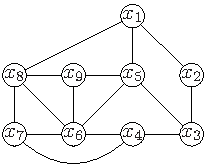
\includegraphics{np-figs/independent3}
  \end{figure}
  \end{frame}

\section{k-Color->SAT}

\begin{frame}
  \frametitle{k-Coloring to SAT}
  \begin{itemize}
  \item Given a graph $G=\langle V,E\rangle$ and $k$-colors 
  \item is it possible to assign a color to every vertex such that no
    two neighbors have the same color?
  \item This is called the $k$-coloring problem
  \item Later we will show that 3-coloring (and thus k-coloring)  is
    NP-complete by reducing 3SAT to 3-Coloring.
  \item Now we need to do the opposite: reduce $k$-coloring to SAT to
    be able to solve $k$-coloring instances.
  \end{itemize}
\end{frame}
\begin{frame}
  \frametitle{Exactly one is true}
  \begin{itemize}
  \item A common occurrence is when we have $k$ variables and we want
   \textbf{ exactly one } of them to be true.
  \item From our previous discussion this is equivalent to 
  \end{itemize}
  \begin{align*}
    (x_1\vee x_2\vee\ldots \vee x_k)\bigwedge_{i\ne j} (\bar{x}_{i}\vee \bar{x}_j)
  \end{align*}
\end{frame}
\begin{frame}
  \begin{itemize}
  \item Let $x_{ij}$, $1\le i\le n$, $1\le j\le k$ be a boolean
    variable such that $x_{ij}=1$ iff node $i$ has color $j$.
  \item Since a node can be assigned exactly one color then: at least
    one is true and at most one is true
  \item Thus for every node $i$ we have a clause:

  \begin{align*}
    (x_{i1}\vee x_{i2}\vee\ldots \vee x_{ik})\bigwedge_{l\ne m} (\bar{x}_{il}\vee \bar{x}_{im})
  \end{align*}
\item Also for every two neighbors $i,j$ cannot have the same color so
  \begin{align*}
    (\bar{x}_{i1}\vee \bar{x}_{j1})\wedge\ldots \wedge (\bar{x}_{ik}\vee \bar{x}_{ik})
  \end{align*}
  \end{itemize} 
\end{frame}
\begin{frame}[fragile]
  \frametitle{Encoding}
  \begin{itemize}
  \item Given $n$ nodes and $k$-colors we encode the variables as follows
  \item the first node we associate nodes $1,\ldots,k$ for the $k$ colors.
  \item The second node  $x_{k+1},\ldots,x_{2k}$
   \item In general for node $i$ we associate the indices $k\cdot i-k+1, k\cdot i-k+2,\ldots,k\cdot i-1$
\item In Python, let colors be an array of colors then the function below returns the variable number for node $i$ color $j$
  \end{itemize}
\begin{lstlisting}[numbers=none]
def varnum(i,j):
  return len(colors)*i-j+1
\end{lstlisting}
\end{frame}

\begin{frame}
  \frametitle{Example}
  \begin{itemize}
    \item Consider again the graph we used to test for independent set and check if it admits 3-coloring. Using z3 we get the solution in the figure below.
    \end{itemize}
  \begin{center}
  \begin{tikzpicture}
    \node[shape=circle,draw=black,fill=green] (x0) at (5,7){$x_0$};
\node[shape=circle,draw=black,fill=blue] (x1) at (8,5){$x_1$};
\node[shape=circle,draw=black,fill=green] (x2) at (8,3){$x_2$};
\node[shape=circle,draw=black,fill=blue] (x3) at (6,3) {$x_3$};
\node[shape=circle,draw=black,fill=blue] (x4) at (6,5) {$x_4$};
\node[shape=circle,draw=black,fill=green] (x8) at (4,5) {$x_8$};
\node[shape=circle,draw=black,fill=blue] (x7) at (1,5) {$x_7$};
\node[shape=circle,draw=black,fill=green] (x6) at (1,3) {$x_6$};
\node[shape=circle,draw=black,fill=red] (x5) at (4,3) {$x_5$};
\path[-,draw] (x0) --  (x1);
\path[-] (x1) edge (x2);
\path[-] (x2) edge (x3);
\path[-] (x3)  edge (x5);
\path[-] (x5)  edge (x6);
\path[-] (x6) edge (x7);
\path[-] (x7)  edge (x8);
\path[-] (x2) edge (x4);
\path[-] (x0) edge (x4);
\path[-] (x0) edge (x7);
\path[-] (x8) edge (x4);
\path[-] (x5) edge (x4);
\path [-] (x5) edge (x8);

\path [-] (x5) edge (x7);
\path [-] (x3) edge[bend left=30] (x6);
%\path [-] (x3) edge[bend left=30] node{$1$} (x6);

    \end{tikzpicture}
  \end{center}

\end{frame}
\begin{frame}
  \frametitle{Mini sudoku}
  \begin{itemize}
  \item Before we use a SAT solver to solve sudoku we try semi-manually to solve a mini version of sudoku
  \item The mini sudoku is just a 2x2 grid. 
  \item As an example consider the grid below
  \end{itemize}
  \begin{center}
  \begin{tikzpicture}
    \draw[step=0.5cm,color=gray] (-1,-1) grid (0,0);
   \node at (-0.75,-0.25) {1};
   \node at (-0.75,-0.75) {2};
  \end{tikzpicture}
  \begin{itemize}
  \item clearly the answer is setting the top white cell to 2 and the bottom to 1
  \item We will see how we encode it as a SAT problem
  \end{itemize}
  \end{center}

\end{frame}
\begin{frame}
  \frametitle{mini sudoku encoding}
  \begin{itemize}
  \item The rules are
    \begin{enumerate}
    \item All cells in the same row cannot have the same value
    \item All cells in the same column cannot have the same value
    \item Each cell can contain only one value
    \end{enumerate}
\item To implement the above we introduce variables $x_{ijk}=1$ if cell $(i,j)$ contains the value $k$. 
   \item For example in the grid above we have $x_{111}=1$ and $x_{212}=1$.
  \end{itemize}
\end{frame}
\begin{frame}
  \begin{itemize}
  \item All cells in row 1  cannot have the same value translates into
    \begin{align*}
      &(x_{111}\vee x_{121})\wedge (\bar{x}_{111}\vee \bar{x}_{121})\\
    \wedge & (x_{112}\vee x_{122})\wedge (\bar{x}_{112}\vee\bar{x}_{122})
    \end{align*}
\item All cells in row 2 cannot have the same value translates into
  \begin{align*}
     &(x_{211}\vee x_{221})\wedge (\bar{x}_{211}\vee \bar{x}_{221})\\
    \wedge & (x_{212}\vee x_{222})\wedge (\bar{x}_{212}\vee\bar{x}_{222})
  \end{align*}
\item All cells in column 1 cannot have the same value translates into
  \begin{align*}
     &(x_{111}\vee x_{211})\wedge (\bar{x}_{111}\vee \bar{x}_{211})\\
    \wedge & (x_{112}\vee x_{212})\wedge (\bar{x}_{112}\vee\bar{x}_{212})
  \end{align*}
\item All cells in column 2 cannot have the same value translates into
  \begin{align*}
     &(x_{121}\vee x_{221})\wedge (\bar{x}_{121}\vee \bar{x}_{221})\\
    \wedge & (x_{122}\vee x_{222})\wedge (\bar{x}_{122}\vee\bar{x}_{22})
  \end{align*}
  \end{itemize}
\end{frame}
\begin{frame}
  \begin{itemize}
  \item Finally, each cell cannot have both values
    \begin{align*}
      (x_{111}\vee x_{112})\wedge (\bar{x}_{111}\vee \bar{x}_{112})\\
      (x_{121}\vee x_{122})\wedge (\bar{x}_{121}\vee \bar{x}_{122})\\
      (x_{211}\vee x_{212})\wedge (\bar{x}_{211}\vee \bar{x}_{212})\\
      (x_{221}\vee x_{222})\wedge (\bar{x}_{221}\vee \bar{x}_{222})\\
    \end{align*}
\item Also $x_{111}=1$ and $x_{212}=1$. 
\item We enter these clauses as input to minisat by renaming the 8 variables as : $x_{111}=1,x_{121}=2,x_{112}=3,x_{122}=4$\\
$x_{211}=5,x_{221}=6,x_{212}=7,x_{222}=8$.
\item The encoding is in the file mini-sudoku.txt on blackboard.
  \end{itemize}
\end{frame}
\begin{frame}[fragile]
  \frametitle{Solving Sudoku}
  \begin{itemize}
  \item Unlike the mini sudoku it is almost impossible to write the needed clauses by hand
  \item We will write a Python code to generate the needed clauses
  \item A central computation that we will need often is when exactly one variable is true
  \item Also we need an automatic encoding of the variables $x_{ijk}$.
  \item We define a function that returns the variable number given $(i,j,k)$ as $100*i+10*j+k$.
  \item In Python
\end{itemize}
\begin{lstlisting}[numbers=none]
def varnum(i,j,k):
   return 100*i+10*j+k
\end{lstlisting}

\end{frame}
\begin{frame}[fragile]
  \begin{itemize}
  \item We define a function that takes an input a list of literals and adds the clauses that guarantees that only one of them is true.
\item Note that below we use the itertools.combinations which returns all combinations of 2 variables from a list of literals.
  \end{itemize}
\begin{lstlisting}[numbers=none]
def exactly_one_of(literals):
    # at least one is true
    solver.add(z3.Or([l for l in literals]))
    # no two can be true
    for u,v in itertools.combinations(literals,2):
        solver.add(z3.Or(z3.Not(u),z3.Not(v)))
\end{lstlisting}
\end{frame}
\begin{frame}
  \begin{itemize}
  \item Using the above we can add the constraints
    \begin{enumerate}
    \item For each cell $(i,j)$ exactly one value is true
   \item For each row value $k$ appears  exactly once
   \item For each column value $k$ appears exactly once
   \item For each 3x3 block value $k$ appears exactly once
   \item Finally, we add the clauses that make the filled cells to be true
    \end{enumerate}
  \end{itemize}
\end{frame}
\begin{frame}
  \frametitle{Dealing with 3x3 blocks}
  \begin{itemize}
  \item Note  the "origin" of each 3x3 block below.
  \item From the "origin" $x$ the block is defined as $(x+\delta_i,x+\delta_j)$ where $\delta_i=0,1,2$ and $\delta_j=0,1,2$.
  \end{itemize}
    \begin{tikzpicture}
    \draw[step=0.5cm,color=gray] (-2,-2) grid (2.5,2.5);
   \node at (-1.75,3) {1};
   \node at (-1.25,3) {2};
   \node at (-0.75,3) {3};
   \node at (-0.25,3) {4};
   \node at (0.25,3) {5};
   \node at (0.75,3) {6};
   \node at (1.25,3) {7};
   \node at (1.75,3) {8};
   \node at (2.25,3) {9};

 \node at (-2.25,-1.75) {9};
   \node at (-2.25,-1.25) {8};
   \node at (-2.25,-0.75) {7};
   \node at (-2.25,-0.25) {6};
   \node at (-2.25,0.25) {5};
   \node at (-2.25,0.75) {4};
   \node at (-2.25,1.25) {3};
   \node at (-2.25,1.75) {2};
   \node at (-2.25,2.25) {1};

\node at (-1.75,2.25) {$x_{11}$};
\node at (-0.25,2.25) {$x_{14}$};
\node at (1.25,2.25) {$x_{17}$};
\node at (-1.75,0.75) {$x_{41}$};
\node at (-0.25,0.75) {$x_{44}$};
\node at (1.25,0.75) {$x_{47}$};

\node at (-1.75,-0.75) {$x_{71}$};
\node at (-0.25,-0.75) {$x_{74}$};
\node at (1.25,-0.75) {$x_{77}$};


  \end{tikzpicture}

\end{frame}
\begin{frame}
  \begin{itemize}
  \item The Python code for the sudoku is on black board
  \end{itemize}
\end{frame}
\begin{frame}
 \frametitle{SAT Modulo Theories}
 \begin{itemize}
  \item A extension of SAT that allows us to reason about other than boolean variables
  \item SMT can be regarded as a constraint satisfaction problem
  \item For example if $x,y,z$ are real numbers or integers 
  \item are the following constraints satisfiable?
  \item $x+y+z=10$
  \item $2\le x\le 7$
  \item $y-z=2$ etc.
   
 \end{itemize} 
\end{frame}

\begin{frame}
  \frametitle{Example: Job Scheduling}
  \begin{itemize}
  \item We will solve an instance of job scheduling using the z3 smt solver
  \item z3 can be used stand alone with input a file in smt-lib format
  \item It also has a binding for other languages C++, C\#, Python
  \end{itemize}
\end{frame}

\begin{frame}
  \frametitle{Example: Job Scheduling}
  \begin{itemize}
    \item Suppose that we have 6 jobs of length (arbitrary units)
    \item $L=[4,5,6,7,8,9]$
    \item Further suppose that you have three workers (A,B and C) 
    referred to as 1,2 and 3 to complete the jobs
    \item Let $s[i],e[i],p[i]$ be the starting time, ending time and the worker that performed job $i$
    \item We have the following constraints
    \item $e[i]-s[i]=L[i]$.
    \item Suppose that job 3 cannot start until jobs 2 and 6 finish 
    \item No worker can perform more than one job at a time
    \item Jobs 1 and 4 require the special skills of worker 2
  \end{itemize}
\end{frame}
\begin{frame}[fragile]
  \frametitle{Example: using z3}
\begin{itemize}
  \item Z3 uses the smt-lib syntax which is very 
  similar to Lisp
  \item First we declare all the needed variables $s,e,p$
\end{itemize}
\begin{verbatim}
  (declare-const s1 Int)
  ...
  (declare-const s6 Int)
  (declare-const e1 Int)
  ...
  (declare-const p6 Int)
\end{verbatim}  

\end{frame}
\begin{frame}[fragile]
  \frametitle{}
\begin{itemize}
  \item Make sure the length of job 1 is 4 and job 2 is 5 etc..
\end{itemize}
\begin{verbatim}
(assert (= e1 (+ s1 4)))
(assert (= e2 (+ s2 5)))
...  
\end{verbatim}  
\begin{itemize}
 \item If jobs 1 and 2 are performed by the same worker make sure that they are
 not done concurrently  
\end{itemize}
\begin{verbatim}
(assert (=> (= p1 p2) (or (>= s1 e2) (>= s2 e1))))
....  
\end{verbatim}
\begin{itemize}
 \item Make sure job 3 cannot start until jobs 2 and 6 finish 
\end{itemize}
\begin{verbatim}
(assert (and (>= s3 e2) (>=s3 e6)))  
\end{verbatim}
\end{frame}
\begin{frame}
  \frametitle{Solution}
  \newcommand*{\TickSize}{2pt}%
  \newcounter{y}
  \setcounter{y}{12}
  \begin{tikzpicture}[scale=0.6]
    
\node at (-12.5,4.25) {$C$};
\node at (-12.5,3.25)  {$B$};
\node at (-12.5,2.25) {$A$};
\node at (-7,4.25) {6};
\node at (0,4.25){3};
\node at (-10,3.25){1};
\node at (-5,3.25){4};
\node at (-9.5,2.25){2};
\node at (-3.8,2.25)  {5}; 
  \draw  (-12,4.5) rectangle (-3,4);
  \draw  (-3,4.5) rectangle (3,4);
  \draw  (-12,3.5) rectangle (-8,3);
  \draw  (-8,3.5) rectangle (-1,3);
  \draw  (-12,2.5) rectangle (-7,2);
  \draw  (-7,2.5) rectangle (1,2);
  \draw (-12,1)--(3,1);
  \foreach \x in {-12,-11,...,3} {%
  \addtocounter{y}{\x}
    \draw ($(\x,1) + (0,-\TickSize)$) -- ($(\x,1) + (0,\TickSize)$)
        node [below] {$\they$};
  \setcounter{y}{12}
  }
  \end{tikzpicture}

  

\end{frame}
\end{document}


%%% Local Variables:
%%% mode: latex
%%% TeX-master: t
%%% End:
